\documentclass{article}
\usepackage[T2A]{fontenc}
\usepackage[utf8]{inputenc}
\usepackage[english, russian]{babel}
\usepackage[left=30mm, right=10mm, top=20mm, bottom=20mm]{geometry}
\usepackage{makeidx}
\usepackage{amsmath}
\usepackage{mathtools}
\usepackage{graphicx}
\graphicspath{{pictures/}}
\usepackage{pgfplots}
\usepackage{amsfonts}
\usepackage[colorlinks=true, allcolors=black]{hyperref}
\usepackage{graphicx}

\begin{document}

\title{Курсовая работа по теме <<Оценка эквивалентных норм>>.}

\author{Пьянков Александр, группа МЕН--390101}

\date{14 июля 2022г.}

\maketitle

\tableofcontents

\newpage
\section{Известные сведения}

Известно, что в любом конечномерном пространстве (которое изомофрно $\mathbb{R}^n$), любые две нормы $\|\cdot\|_1, \|\cdot\|_2$ эквивалентны, т.е.

$$ \exists \alpha, \beta > 0 \, \forall x \in X = \mathbb{R}^n: \; \alpha\|x\|_1 \leq \|x\|_2 \leq \beta \|x\|_1. $$

\textbf{Текущая задача} состоит в поиске величины $ C = \sup\limits_{x \neq 0} \frac{\|x\|_1}{\|x\|_2}$ и элемента $x^*$, на котором эта величина достигается.

Ее можно рассматривать как норму функционала $\|\cdot\|_1$ на пространстве $(\mathbb{R}^n, \|\cdot\|_2).$

Она достигнется обязательно, т.к. ее можно рассматривать на единичной сфере по $\|\cdot\|_2$: 

$$ C = \sup\limits_{\|x\|_2=1}{\|x\|_1}. $$
Такая сфера в конечномерном пространстве -- компакт, а функция $\|\cdot\|_1$ непрерывна, по теореме Вейерштрасса достигнется величина $C$, причем в силу четности нормы $(\forall \|\cdot\|: \; \|x\| = \|-x\|)$, элементов $x^*$ будет четное число.

\newpage
\section{Некоторые частные случаи}

\subsection{p-нормы в пространствах n-мерных векторов}

Для любых норм вида $ \|x\|_p = \sqrt[p]{\sum\limits_{i=1}^n{|x_i|^p}}, \; 1 \leq p < \infty $, величина $C = 1$ и достигается на элементе $x^*=(1,0,...,0)$:

$$ \|(1,0,...,0)\|_p = 1 = \|(1,0,...,0)\|_q \; \forall p,q \in [1,\infty), $$ 
если только $q < p$, т.к. при этом обязательно будет неравенство $\|x\|_p \leq \|x\|_q$. (См. ~\cite{Zorich2}, c. 42). Это соотношение следует из вложенности единичных шаров норм такого вида -- чем больше $p$, тем больше шар $\|x\|_p = 1$, однако точки, лежащие на осях координат и имеющие единичную норму, будут принадлежать всем единичным шарам, изобразим такое вложение при $n=2$ и различных $p$:
\begin{center}
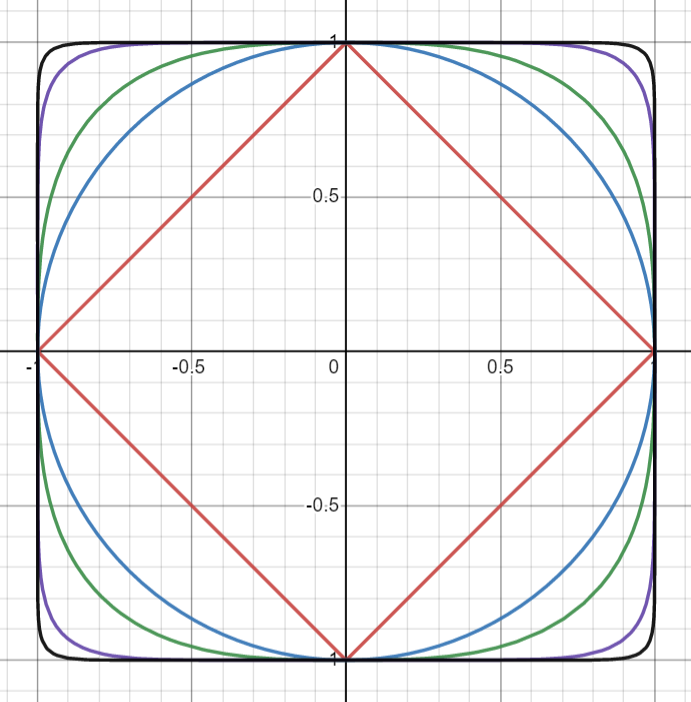
\includegraphics[scale=0.8]{pictures/p_spheres.png}
\end{center}
Теперь предположим, что $1 \leq p < q < \infty. $ Можно преобразовать выражение величины $C$:
$$ C = \sup\limits_{\|x\|_q=1}{\|x\|_p}. $$
Рассмотрим единичную сферу по норме с индексом $q$ : $ S_q[0,1] = \{x: \|x\|_q = 1\}.$ На ней
$$\exists x^*: \|x^*\|_q = 1, \, C = \|x^*\|_p = \max\limits_{\|x\|_q=1}{\|x\|_p}.$$
Рассмотрим точки, у которых модули всех координат равны, таких точек $x^*$ на анализируемой сфере будет $2^n$, где $n$ -- размерность пространства. Для наглядности покажем изображение при $n=2$:

\vspace{2mm}
\begin{center}
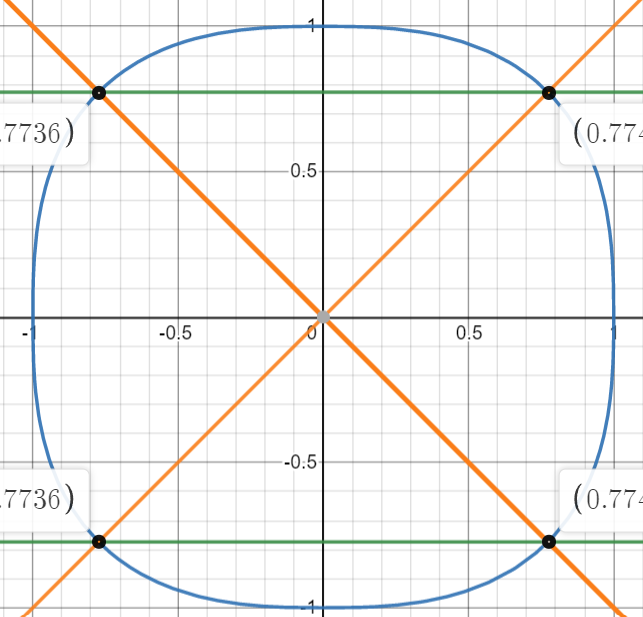
\includegraphics[scale = 0.8]{p_norms.png}
\end{center}
\vspace{2mm}

Ровно одна из них будет иметь координаты вида $x^* = (a,a,...,a), \, a > 0.$ Найдем $a$:
$$ 1 = (n(a^q))^\frac{1}{q} \Rightarrow a = \frac{1}{n^\frac{1}{q}} \Rightarrow C \geq \|x^*\|_p = \left(n^{\frac{-p}{q}} \cdot n\right)^{\frac{1}{p}} = n^{\frac{1}{p}-\frac{1}{q}}. $$
Теперь оценим $C$ сверху. Согласно неравенству Гельдера, 
$$ \|x\|_p^p = \sum\limits_{i=1}^n|x_i|^p = \sum\limits_{i=1}^n(|x_i|^p \cdot 1) \leq \left(\sum\limits_{i=1}^n(|x_i|^p)^{\frac{q}{p}}\right)^{\frac{p}{q}} \cdot \left(\sum\limits_{i=1}^n 1^{\frac{q}{q-p}}\right)^{\frac{q-p}{q}} = $$
$$ = \|x\|_q^p \cdot n^{1-\frac{p}{q}} \Rightarrow \|x\|_p \leq \|x\|_q \cdot n^{\frac{1}{p}-\frac{1}{q}}. $$

Аналогично показываются оценки (и они будут теми же), когда $p$ или $q$ равны $\infty$.

Подводя итог, 
\begin{equation*} C = C_{p,q} = 
	\begin{cases}
		1 & q \leq p; \\
		n^{\frac{1}{p}-\frac{1}{q}} & q > p.
	\end{cases}
\end{equation*}
\begin{equation*} x^* = x_{p,q}^* = 
	\begin{cases}
		(1,0,...,0) & q \leq p; \\
		\left(n^{\frac{-1}{q}}, n^{\frac{-1}{q}},..., n^{\frac{-1}{q}} \right) & q > p.
	\end{cases}
\end{equation*}

\subsection{Ромбические нормы}
Пусть пока $n=2$. Рассмотрим набор положительных чисел $a=(a_1, a_2)$ и ромбическую норму $\|x\|_a = a_1|x_1|+a_2|x_2|$. Единичной сферой по этой норме будет ромб

\begin{center}
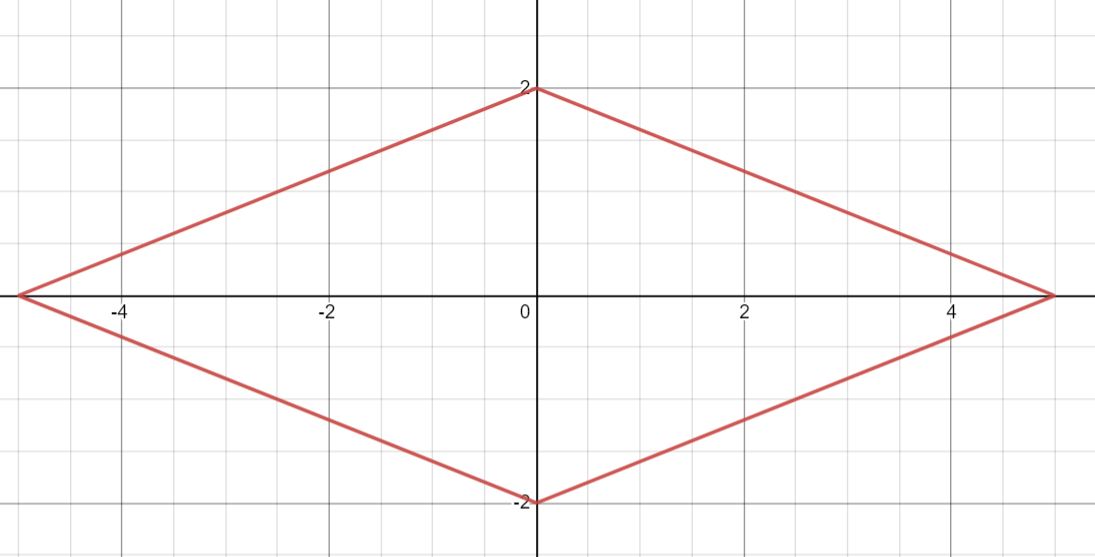
\includegraphics[scale = 0.45]{rhombus.png} 
\end{center}

Возьмем еще один набор положительных чисел $b = (b_1, b_2)$. Пусть элемент $x \in \mathbb{R}^2$ такой, что $\|x\|_b = b_1|x_1|+b_2|x_2| = 1$. Для решения исходной задачи нужно найти максимум величины $\|x\|_a$ и экстремального элемента $x^*$, на котором он достигается. Имеем

$$ \|x\|_a = a_1|x_1| + a_2|x_2| = \frac{a_1}{b_1}(1-b_2|x_2|) + a_2|x_2| =: f(x_2), \; \text{б.о.о.,} \; x_2 \geq 0. $$

Найдем производную: 

$$ f'(x_2) = a_2 - \frac{a_1b_2}{b_1}. $$

Если она равна нулю, то функция $f$, она же -- норма $\|x\|_a$ не зависит от $x$ при $\|x\|_b = 1$, т.е. ромбы (единичные шары) будут масштабированы относительно точки $0$. Тогда искомая величина достигается на любом $x \neq 0$ и равна $ \frac{a_1}{b_1} = \frac{a_2}{b_2}$.

Пусть теперь производная не равна нулю, тогда функция $f$ линейна, следовательно достигает экстремума на концах отрезка ее определения $[0, t].$ Найдем $t$ ($x_1$ -- абсцисса, $x_2$ -- ордината):

$$ x_2 = t \Leftrightarrow x_1 = 0, \; b_1 \cdot 0 + b_2 \cdot t = 1 \Rightarrow t = \frac{1}{b_2}.$$

$$ f(0) = \frac{a_1}{b_1}, \, f\left(\frac{1}{b_2}\right) = \frac{a_2}{b_2}. $$

В любом случае получили ответ
$$ C = \max\left(\frac{a_1}{b_1}, \frac{a_2}{b_2}\right), $$
при $x_2 \geq 0$. Аналогично можно показать, что при $x_2 \leq 0$ ответ не изменится в силу симметрии ромба. Экстремальный элемент будет таковым:

\begin{equation*} x^* = 
	\begin{cases}
		\left(\frac{1}{b_1},0\right) & \frac{a_1}{b_1} \geq \frac{a_2}{b_2}; \\
		\left(0,\frac{1}{b_2}\right) & \frac{a_2}{b_2} \geq \frac{a_1}{b_1}.
	\end{cases}
\end{equation*} 

При этом этот же ответ покроет случай пропорциональности ромбов. Если $n > 2$, то ответ будет аналогичен:
$$ C = \max\limits_{i=\overline{1,n}}\frac{a_i}{b_i}, \; x^* = \left(0,0,...,\frac{1}{b_i},...,0\right), $$
где $i$ -- индекс максимума отношения $\frac{a_i}{b_i}$.

Немного поясним этот ответ. <<Вкладывая>> всю ненулевую часть элемента в индекс максимума отношения, искомая величина окажется наибольшей, из-за линейной суммы формулы ромбической нормы (без степеней координат, т.е. суммы модулей координат с весами $a_i$, $b_i$). То есть нужно полностью <<вложиться>> в наибольшее отношение этих весов, тогда получится максимальный результат. Упрощенный пример: пусть $m > n > 0$ и нужно подобрать числа $a, b : \; a, b > 0, \, a + b = 1$ такие, что $am+bn$ максимально. Очевидно, что $a=1, b=0$, т.е. в наибольший вес $m$ полностью вложили все допустимые данные из $a, b$. Однако при наличии степеней в формуле нормы это не так.

\subsection{Прямоугольные нормы}

Это нормы вида $\|x\|_a = \max\limits_{i=\overline{1,n}}(a_i|x_i|), \; a_i > 0, \; a = (a_1,...,a_n) \text{ -- набор чисел.}$ Единичная сфера по этой норме -- $n$-мерный прямоугольник со сторонами, параллельными осям координат, с центром в точке (0,0,...,0). Для двух таких норм $\|x\|_a, \|x\|_b$ найдем искомую величину: пусть $\|x\|_b = 1, \; j$ -- индекс, на котором $ \|x\|_b = b_j|x_j| = 1 \Rightarrow |x_j| = \frac{1}{b_j}, \; \forall{i \neq j}: |x_i| \leq \frac{1}{b_i}$ , тогда имеем
$$ \exists{k \in \{1,2,...,n\}}: \|x\|_a = a_k|x_k| \leq \frac{a_k}{b_k}, $$
причем равенство достигнется например при $ x^* = \left(0,0,...,\frac{1}{b_k},...,0\right)$, и $ C = \|x^*\|_a = \frac{a_k}{b_k}$, где $k$ таково, что 
$$ \|x^*\|_a = \max\limits_{i=\overline{1,n}}(a_i|x_i^*|) \leq \max\limits_{i=\overline{1,n}}\frac{a_i}{b_i} = a_k|x_k^*| = \frac{a_k}{b_k}. $$ 
Оценка для $C$ получилась такой же, что и для ромбических норм, причем можно брать тот же вектор $x^*$. 

\newpage
\section{Оценка на плоскости} \label{3}

Здесь $n=2$, координаты $(x,y)$. Предположим, что формулы норм $f = \|\cdot\|_1, \, g = \|\cdot\|_2$ -- достаточно гладкие функции. Будем рассматривать функцию $f$ на единичной сфере $g(x,y) = \|(x,y)\|_2 = 1$. Задача свелась к нахождению условного экстремума (точнее -- максимума) функции многих переменных. Она решается методом множителей Лагранжа.

Условие связи одно: $g(x,y) = 1 \Leftrightarrow \varphi(x,y) = g(x,y) - 1 = 0$, функция Лагранжа имеет вид:
$$ L(x,y) = f(x,y) + \lambda \cdot (g(x,y) - 1) $$
Для достижения экстремума необходимо, чтобы $L'_x = L'_y = L'_{\lambda} = 0$. Подставим:
\begin{equation}\label{eq:l2}
	\begin{cases}
		f'_x(x,y)+\lambda g'_x(x,y) = 0; \\
		f'_y(x,y)+\lambda g'_y(x,y) = 0; \\
		g(x,y) = 1.
	\end{cases}
\end{equation}
Дальнейшие рассуждения требуют конкретики от функций $f, g$. Однако можно отметить важный частный случай, в котором частные производные функций-норм не обращаются в 0:
$$ -\lambda = \frac{f'_x}{g'_x} = \frac{f'_y}{g'_y}. $$
То есть точки экстремума характеризуются равенством отношений частных производных функций-норм по одной и той же переменной. Такое свойство экстремальности точек справедливо и для произвольной конечной размерности $n$ пространства.
\subsection{Эллиптические нормы}
Это нормы вида $\|x\|_a = \sqrt{\sum\limits_{i=1}^n a_i|x_i|^2}, \; \forall{i=\overline{1,n}}: a_i > 0, \; a = (a_1,...,a_n)$. Нарисуем единичную сферу на плоскости для нормы этого типа:

\begin{center}
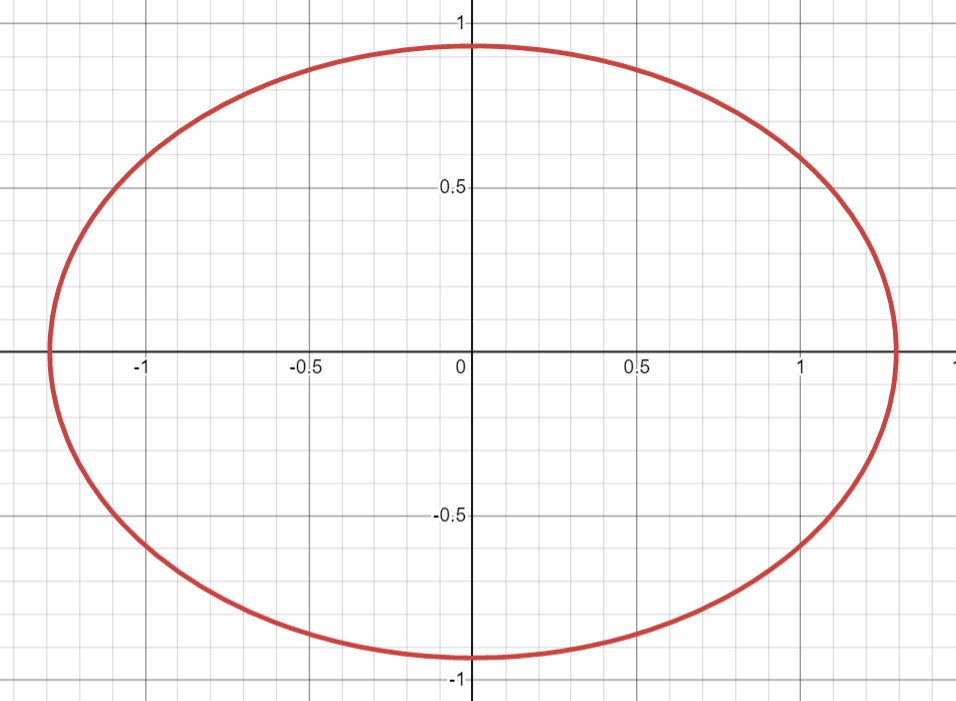
\includegraphics[scale=0.55]{ellipse.png} 
\end{center}

Пусть $f(x,y) = \sqrt{ax^2+by^2}, \; g(x,y) = \sqrt{cx^2+dy^2}, \; a,b,c,d > 0$ - две эллиптические нормы. Подставим их в \eqref{eq:l2}:
\begin{equation*}
	\begin{cases}
		\frac{ax}{\sqrt{ax^2+by^2}}+\lambda \left( \frac{cx}{\sqrt{cx^2+dy^2}} \right) = 0; \\
		\frac{by}{\sqrt{ax^2+by^2}}+\lambda \left( \frac{dy}{\sqrt{cx^2+dy^2}} \right) = 0; \\
		cx^2+dy^2 = 1.
	\end{cases}
\end{equation*}
Рассмотрим 3 случая.
\vspace{1mm}

1) $x = 0 \Rightarrow y = \pm\sqrt{1/d}, \; f(x,y) = \sqrt{b/d}. $

2) $y = 0 \Rightarrow x = \pm\sqrt{1/c}, \; f(x,y) = \sqrt{a/c}. $

3) $x \cdot y \neq 0$. Тогда
$$ \lambda = \frac{-ax}{cx\sqrt{ax^2+by^2}} = \frac{-by}{dy\sqrt{ax^2+by^2}} \Rightarrow \frac{a}{c} = \frac{b}{d}. $$ 
В таком случае нормы будут пропорциональны, их эллипсы (единичные сферы) -- подобны, и искомая величина достигнется в любой ненулевой точке. Она будет равна $C = \sqrt{a/c} = \sqrt{b/d}$.

В итоге, независимо от номера случая, получилось, что $$ C = \max\left(\sqrt{\frac{a}{c}}, \sqrt{\frac{b}{d}}\right); $$
\begin{equation*} \big((x,y)\big)^* =
	\begin{cases}
		\left(\frac{1}{\sqrt{c}}, 0\right), & \frac{a}{c} \geq \frac{b}{d}; \\
		\left(0, \frac{1}{\sqrt{d}}\right), & \frac{a}{c} < \frac{b}{d}.
	\end{cases}
\end{equation*}
\vspace{1mm}

\subsection{Произвольная и евклидова норма}
Пусть $f(x,y)$ -- произвольная норма на $\mathbb{R}^2$, $\forall{x,y \in \mathbb{R}^2} \,\exists{f'_x(x,y), f'_y(x,y)}$, \newline $g(x,y) = \sqrt{x^2+y^2} $ -- евклидова норма. Тогда нас интересуют точки $(x,y)$, в которых $g(x,y)^2 = x^2 + y^2 = 1$. Подставим имеющиеся данные в соотношения \eqref{eq:l2}:
\begin{equation*}
	\begin{cases}
		f'_x(x,y) + \lambda x = 0; \\
		f'_y(x,y) + \lambda y = 0; \\
		x^2 + y^2 = 1.
	\end{cases}
\end{equation*}
Отсюда, обозначив $f'_x(x,y) = a, \; f'_y(x,y) = b$:
$$ x = \frac{-a}{\lambda}, \; y = \frac{-b}{\lambda}, \; a^2 + b^2 = \lambda^2; $$
$$ \lambda = \pm \sqrt{a^2+b^2}, \; x = \pm\frac{-a}{\sqrt{a^2+b^2}}, \; y = \pm\frac{-b}{\sqrt{a^2+b^2}}. $$
Всего получилось 4 точки (все возможные комбинации знаков $+$ и $-$ в $x,y$), причем из соображений симметрии, в двух из них достигнется минимум, в двух других -- максимум. Кроме того, экстремумы будут распределены по этим точкам следующим образом:
 
\vspace{1mm}
1) $x, y$ взяты с плюсом -- это точка максимума, и во второй точке максимума обе координаты взяты с минусом. Две других комбинации знаков дадут две точки минимума.

2) Точки максимума характеризуются разными знаками координат $x,y$, минимума -- одинаковыми.

\vspace{1mm}
Искомая величина $C$ достигнется в точках максимума.

Полученный вывод можно обобщить и на $n$-мерное пространство: пусть $f(x_1,...,x_n)$ -- произвольная норма на $\mathbb{R}^n$, $g(x_1,...,x_n) =  \sqrt{\sum\limits_{i=1}^n{x_i^2}}$ -- евклидова норма. Тогда экстремальные точки будут равны
$$ x_i = \pm \frac{-a_i}{\sqrt{\sum\limits_{j=1}^n{a_j^2}}} = \pm \frac{-a_i}{g(a_1,...,a_n)}, \; a_i = \frac{\partial f}{\partial x_i}, \; i=1,...,n. $$

\subsection{Исследование сфер} \label{3.3}
Обозначим $S_R(\|\cdot\|)$ -- сфера радиуса $R$ нормы $\|\cdot\|$, т.е. множество точек $(x,y) \in \mathbb{R}^2$ таких, что $\|(x,y)\| = R$. Пусть $f,g$ -- две произвольные нормы на $\mathbb{R}^2$, тогда сферы $S_r(f), \, S_R(f), \, S_1(g)$ будут выглядеть так:

\vspace{2mm}
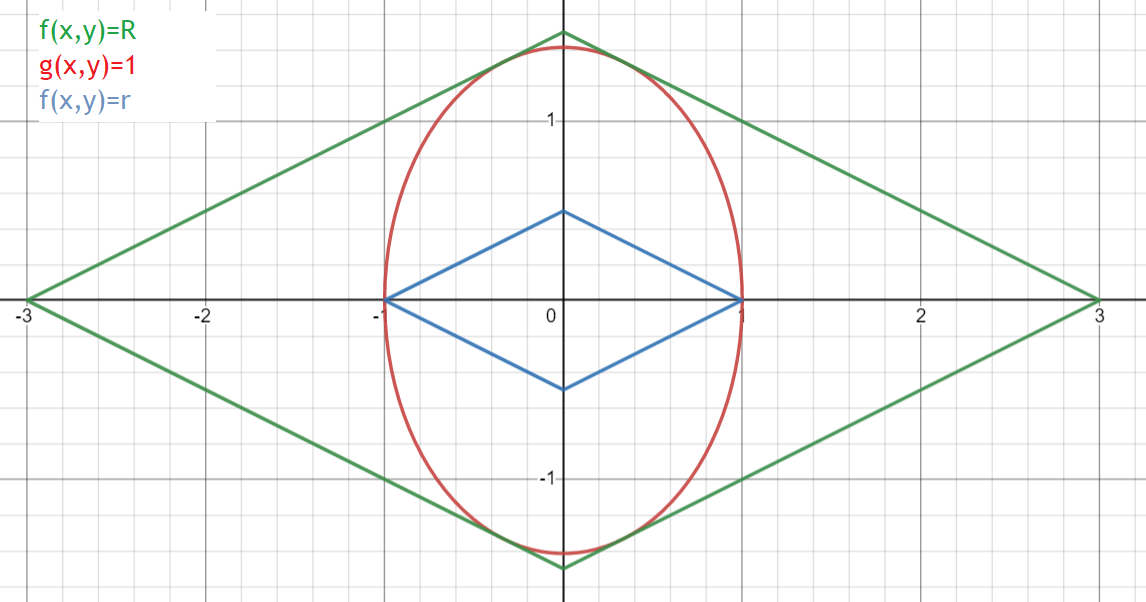
\includegraphics[scale=0.4]{pictures/spheres.png}

Экстремальными для отношения $ \frac{f(x,y)}{g(x,y)} $ являются точки, лежащие на 2-х сферах одновременно, при этом одна сфера должна быть целиком вложена в другую, как на рисунке выше. Более того, если $S_r(f) \subseteq S_1(g) $, то точки, принадлежащие этим сферам будут точками минимума отношения $ \frac{f(x,y)}{g(x,y)} $, равного $r$; а при $S_1(g) \subseteq S_R(f) $ соответствующие точки будут являться точками максимума этого отношения, равного $R$, который является искомой величиной.

Такое исследование подлежит обобщению на $n$-мерное пространство: в том случае соотношения между вложенностью сфер и соответствующим экстремумом сохранятся.

\subsection{Применение дифференциальной геометрии} \label{3.4}
Дана норма $f(x,y)$ на плоскости $\mathbb{R}^2$. Предположим, что сфера $S_1(f)$ имеет параметризацию
\begin{equation*}
	\begin{cases}
		x = x(t); \\
		y = y(t); \\
		t \in [0, T], \; T \text{ -- период: } x(T) = x(0), \; y(T) = y(0).
	\end{cases}
\end{equation*}
Также для гладкости функции $f$ необходимо условие на параметризацию: $|x'(t)| + |y'(t)| > 0$. В точках экстремума отношения $f/g$, где $g$ -- евклидова норма на $\mathbb{R}^2$, параметризованная сфера касается окружности, причем, согласно разделу \ref{3.3}, положение окружности внутри кривой соответствует максимуму указанного отношения; снаружи -- минимуму. Изобразим случай максимума отношения $f/g$: 
\begin{center}
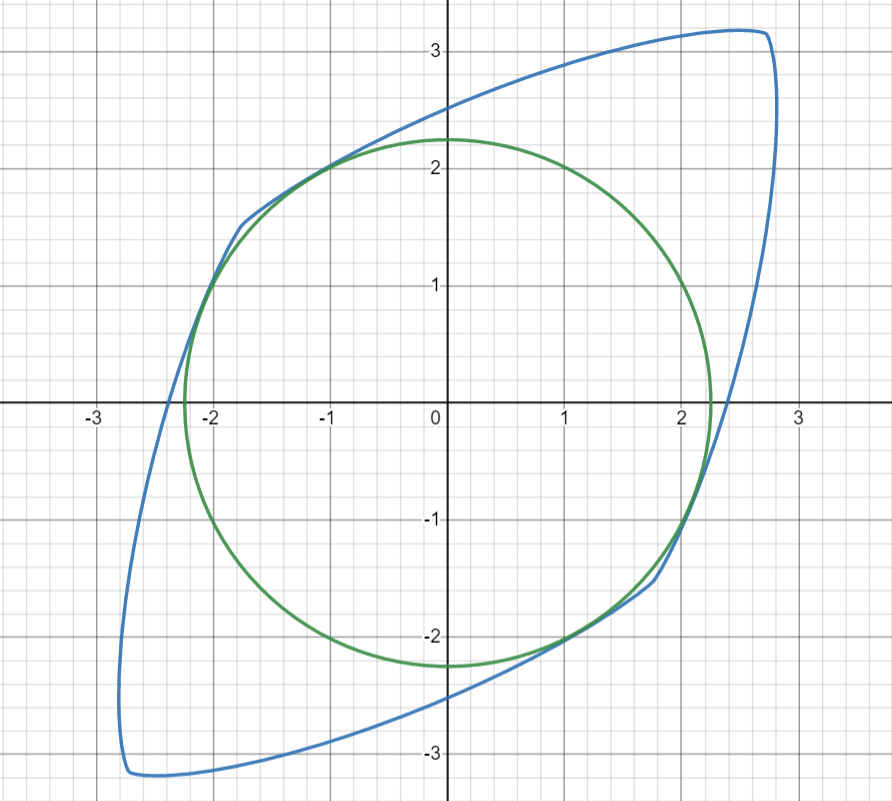
\includegraphics[scale=0.55]{pictures/s1f_circle.png}
\end{center}
Искомые точки, они же -- точки касания двух кривых (окружности и параметризованной сферы), обладают свойством, что нормаль к параметризованной кривой равна нормали к окружности, потому что в этих точках касательная к окружности и сфере $S_1(f)$ общая, следовательно и нормаль тоже общая, или, по крайней мере, эти нормали коллинеарны.
Кроме того, поскольку в любой точке окружности касательная ортогональна радиусу, а нормаль по определению ортогональна касательной, то для каждой точки окружности выполняется свойство коллинеарности нормали в этой точке ее радиус-вектору.
Направляющий вектор касательной при некотором $t \in [0, T]$ (см. \cite{Ignatyev}, с. 27) задается формулой $(x'(t), y'(t))$, следовательно, нормаль можно задать как $(-y'(t), x'(t))$. Тогда необходимое условие можно записать так:
\begin{equation} \label{eq:3.4}
\frac{x(t)}{-y'(t)} = \frac{y(t)}{x'(t)} \Rightarrow x(t)x'(t) + y(t)y'(t) = 0.
\end{equation}
Дальнейшие действия требуют конкретной формулы параметризации (например $x(t) = 0.4\sin{t}, y(t) = \cos{t}$), вследствие которой решается нелинейное в общем случае уравнение для поиска $t$, затем каждый найденный корень $t_0$ подставляется сначала в параметризацию, потом вычисляется евклидова норма точки
\newline 
$(x(t_0), y(t_0))$. Ответом к поставленной в начале работы задаче является точка минимума евклидовой нормы (ей соответствует один из корней уравнения \eqref{eq:3.4}) и величина, обратная этому минимуму (т.к. требуется найти $\max{(f/g)}$, при котором $f=1$).

\vspace{1mm}
Таким образом, уравнение \eqref{eq:3.4} характеризует точки экстремума отношения норм, одна из которых -- евклидова, а другая имеет параметризацию $x(t), \, y(t), \; t \in [0, T] $.

\subsection{Две произвольные нормы} \label{3.5}
Пусть теперь $f, \, g$ -- две произвольные нормы достаточной гладкости. Сделаем невырожденную замену переменных необходимой гладкости, переводящая норму $g$ в евклидову (такая замена существует, т.к. единичный шар по любой норме -- замкнутое, поглощающее, ограниченное множество, следовательно между двумя такими множествами существует \textit{гомеоморфизм}, которым является рассматриваемая замена):
\begin{equation*}
	\begin{cases}
		\tilde{x} = \tilde{x}(x, y); \\
		\tilde{y} = \tilde{y}(x, y); \\
		g(\tilde{x}, \tilde{y}) = g(\tilde{x}(x,y), \tilde{y}(x,y)) = \tilde{g}(x,y) = \sqrt{x^2+y^2}.
	\end{cases}
\end{equation*}
Тогда норма $f$ также преобразуется: $f(\tilde{x}, \tilde{y}) = f(\tilde{x}(x,y), \tilde{y}(x,y)) = \tilde{f}(x,y)$, но главное, что удалось преобразовать одну норму в евклидову, а этот случай был рассмотрен в предыдущем разделе, т.е. точка экстремума $(x,y)$ отношения $\tilde{f}/\tilde{g}$ характеризуется уравнением
$x(t)x'(t) + y(t)y'(t) = 0$, где $t$ -- переменная параметризации единичной сферы нормы $ \tilde{f}$. Схема решения следующая: находим корни уравнения \eqref{eq:3.4}, подставляем их в параметризацию сферы для нормы $ \tilde{f}$, затем вычисляем их евклидову норму (значение функции $\tilde{g}$ в них), выбираем наибольшее и наименьшее из получившихся значений (фиксируя точки $(x(t),y(t)) = (x,y)$ этих экстремумов). Однако получившиеся точки не нужно подставлять в уравнения замены переменных и затем считать от результата замены исходные нормы, т.к. исходные нормы, аргументы которых -- замененные переменные, перешли в параметризованную и евклидову нормы, аргументами которых являются незамененные переменные.

\vspace{1mm}
В заключении стоит отметить, что рассуждения, приведенные в разделах \ref{3.4}, \ref{3.5} также подлежат обобщению на случай $n$-мерного пространства, но тогда условие коллинеарности нормали радиус-вектору будет выглядеть иначе, поскольку нормаль задается иным способом. Однако рассуждения текущего раздела справедливы для любого конечномерного пространства, замена переменных очевидна:
\begin{equation}\label{replace}
	\begin{cases}
		\tilde{x}_1 = \tilde{x}_1(x_1,x_2,...,x_n); \\
		\tilde{x}_2 = \tilde{x}_2(x_1,x_2,...,x_n); \\
		... \\
		\tilde{x}_n = \tilde{x}_n(x_1,x_2,...,x_n); \\
		g(\tilde{x}_1, \tilde{x}_2, ..., \tilde{x}_n) = \sqrt{\sum\limits_{k=1}^n{x_k^2}}.
	\end{cases}
\end{equation}

\newpage
\section{Общий случай}
Рассуждения для некоторых пар норм из раздела \ref{3} обобщаются на этот случай, это было указано после рассмотрения таких пар в 2-мерном пространстве.
\subsection{Анализ нормали}
Даны две нормы $f, \, g$ на пространстве $\mathbb{R}^n$ достаточной гладкости. Благодаря выводу из раздела \ref{3.5}, достаточно рассмотреть случай, когда одна из норм -- евклидова. Пусть ей является норма $g$ для определенности. Для сферы в $\mathbb{R}^n$ справедливо то же свойство, связанное с нормалью, что и для окружности: нормаль, исходящая из точки сферы коллинеарна радиус-вектору этой точки. Согласно заключению в разделе \ref{3.3} справедливы рассуждения относительно вложенности сфер -- единичной для нормы $f$ и масштабируемой для нормы $g$. \vspace{1mm} \newline
Параметризация $n-1$-мерной поверхности в $\mathbb{R}^n$ (коей является сфера для нормы) записывается в неявном виде $F(x_1,x_2,...,x_n) = 0$. Однако поскольку для точек $(x_1,x_2,...,x_n)$ этой сферы выполнено $f(x_1,x_2,...,x_n) = 1$, то $F = f - 1$.
Запишем уравнение нормали к поверхности $F = 0$ (по аналогии с \cite{Ignatyev}, c. 28-30), проведенной к точке $x^{(0)} = \left(x_1^{(0)},x_2^{(0)},...,x_n^{(0)}\right)$:
$$ \frac{x_1-x_1^{(0)}}{\frac{\partial F}{\partial x_1}\left(x^{(0)}\right)} = \frac{x_2-x_2^{(0)}}{\frac{\partial F}{\partial x_2}\left(x^{(0)}\right)} = ... = \frac{x_n-x_n^{(0)}}{\frac{\partial F}{\partial x_n}\left(x^{(0)}\right)}. $$
В знаменателях этих дробей стоят координаты направляющего вектора нормали (т.е. коллинеарного ей). Обозначив $\forall{i = \overline{1,n}} \; A_i := \frac{\partial F}{\partial x_i}\left(x^{(0)}\right) = \frac{\partial f}{\partial x_i}\left(x^{(0)}\right)$, свойство точек на сфере представится в виде
$$ \frac{A_i}{x_i^{(0)}} = C, \; i = \overline{1,n}. $$
\vspace{2mm}
\newline
\textbf{Вывод:} искомые точки экстремума отношения норм $f/g$ характеризуются одинаковым отношением частной производной функции $f$ по $i$-й переменной в этой точке к $i$-й координате этой точки.
\vspace{2mm}
\newline
Поясним, что значит необходимая гладкость функций $f$ и $g$. Поскольку случай, рассмотренный в разделе \ref{3} обобщается здесь, и здесь требуется существование первых производных функции $f$, а у евклидовой нормы существуют производные любого порядка (кроме точки 0, но через нее не проходит ни одна единичная сфера), то этой гладкостью является однократная дифференцируемость функций $f,g$ и однократная дифференцируемость, отсюда же -- непрерывность замены \eqref{replace}.

\subsection{Пространство тригонометрических многочленов}
Вид тригонометрического многочлена $n$-го порядка: 
$$T_n(x) = \frac{a_0}{2} + \sum\limits_{k=1}^n {a_k\cos{kx} + b_k\sin{kx}}$$.
Он определен при всех $x \in \mathbb{R}$ и непрерывен на действительной оси, поэтому будем рассматривать тригонометрические многочлены для всех $x \in \mathbb{R}$. Пространство тригонометрических многочленов $n$-го порядка обозначается $\mathbb{T}_n$, стандартным базисом которого является система функций $\Phi = \left\{\frac{1}{\sqrt{2}},\cos{x},\sin{x},...,\cos{nx},\sin{nx}\right\}$. На этом пространстве, как и на любом конечномерном линейном, можно задать норму. Наиболее распространенные и используемые из них имеют вид (\cite{Tikhomirov}, с. 56-57)
$$ \|T_n\|_p = \left(\frac{1}{\pi}\int\limits_{-\pi}^{\pi}{|T_n(x)|^pdx} \right)^{\frac{1}{p}}, \; p \geq 1. $$
Отметим также норму при $p=\infty$
$$ \|T_n\|_{\infty} = \text{ess}\sup\limits_{x \in \mathbb{R}} {|T_n(x)|} = \sup\limits_{x \in \mathbb{R}} {|T_n(x)|} = \max\limits_{-\pi \leq x \leq \pi} {|T_n(x)|}. $$
Наибольшее применение, особенно в рядах Фурье, (см. \cite{Kolmogorov}, с. 425) имеет норма при $p = 2$:
$$ \|T_n\|_2 = \sqrt{\frac{1}{\pi}\int\limits_{-\pi}^{\pi}{(T_n(x))^2dx}}. $$
По этой норме можно ввести скалярное произведение в пространстве $\mathbb{T}_n$:
$$ \langle f, g \rangle = \frac{1}{\pi}\int\limits_{-\pi}^{\pi}{f(x)g(x)dx}, $$
тогда вышеупомянутая система функций $\Phi$ будет ортонормальной, т.е. 
$$\forall{\varphi_1,\varphi_2 \in \Phi} \, (\varphi_1 \neq \varphi_2 \Rightarrow \langle \varphi_1, \varphi_2\rangle = 0); \, \forall{\varphi \in \Phi}: \, \langle \varphi, \varphi \rangle = 1.$$

\vspace{3mm}
Перейдем к оценке норм $\|\cdot\|_p, \|\cdot\|_q; \text{ для простоты } 1 \leq p < q < \infty$. Нам предстоит оценить выражение $\frac{\|T_n\|_p}{\|T_n\|_q}$. Для этого воспользуемся интегральным неравенством Гельдера с показателями $\frac{q}{p}$ и $\frac{q}{q-p}$. Оба показателя при наложенных на $p$ и $q$ ограничениях попадают в диапазон от $1$ до $\infty$, что свидетельствует о легитимности применения указанного неравенства.
$$ \|T_n\|_p^p = \frac{1}{\pi}\int\limits_{-\pi}^{\pi}{|T_n(x)|^p \cdot 1dx} \leq \frac{1}{\pi}\left(\int\limits_{-\pi}^{\pi}{|T_n(x)|^{p\cdot\frac{q}{p}}dx}\right)^{\frac{p}{q}}\left(\int\limits_{-\pi}^{\pi}{1^{\frac{q}{q-p}}dx}\right)^{\frac{q-p}{q}} = $$
$$ = \left(\frac{1}{\pi}\right)^{1-\frac{p}{q}}\|T_n\|_q^p\left(2\pi\right)^{1-\frac{p}{q}}. $$
Получаем следующую оценку:
$$ \|T_n\|_p \leq \|T_n\|_q\cdot 2^{\frac{1}{p}-\frac{1}{q}}. $$
Причем равенство достигается например при $T_n(x) \equiv 1$, т.к. $\forall{p \in [1,\infty)}: \, \|1\|_p = 2^{\frac{1}{p}}$.
\newline
Итак, искомая величина $C$ равна $ 2^{\frac{1}{p}-\frac{1}{q}}$, а экстремальный элемент $T_n(x) \equiv 1$. Очевидно, что при $q=\infty$ ответ остается справедливым: $\|T_n\|_p \leq \|T_n\|_{\infty} \cdot 2^{\frac{1}{p}}, \; \|1\|_{\infty} = 1$.

\newpage
\section{Заключение}
Оценка отношения двух эквивалентных норм, или любых двух норм в конечномерном пространстве позволяет понять, насколько сильно масштабированы и искажены единичные шары этих норм. Поскольку единичный шар любой нормы в конечномерном пространстве -- множество поглощающее, то зафиксировав шар одной нормы и масштабируя другой, можно добиться их внутреннего и внешнего касания, которые будут соответствовать двум противоположным экстремумам отношения этих двух норм, например внутреннее касание соответствует минимуму, внешнее -- максимуму. При этом точки касания получившихся шаров будут точками достижения этих экстремумов.
\newline
В некоторых случаях, например когда известно, что формулы норм имеют достаточную гладкость, например дифференцируемость, удобно применить ее к исследованию экстремумов и соответствующих им точек. А применяя дифференциальную геометрию конечномерного пространства, можно получить интересный результат: в точках экстремума отношения произвольной нормы к евклидовой вектор-градиент функции, задающей эту произвольную норму, коллинеарен радиус-вектору этой точки.

\newpage
\begin{thebibliography}{9}
\bibitem{Zorich2}
Зорич В. А. <<Математический анализ>>, часть 2. Издание 9-е, исправленное. --- Москва, МЦНМО, 2019. --- 676 с.
\bibitem{Ignatyev}
Игнатьев Ю. Г. <<Дифференциальная геометрия кривых и поверхностей в еквлидовом пространстве>>. Учебное пособие, 4-й семестр. --- Казань, Казанский университет, 2013. --- 204 с.
\bibitem{Tikhomirov}
Тихомиров В. М. <<Математическое просвещение>>. Третья серия, вып. 9. --- Москва, МЦНМО, 2005. --- 240 с.
\bibitem{Kolmogorov}
Колмогоров А. Н., Фомин С. В. <<Элементы теории функций и функционального анализа>>. 7-е издание. --- Москва, ФИЗМАТЛИТ, 2004. --- 572 с.
\end{thebibliography}
\end{document}